%----------------------------------------
% Write your notes here
%----------------------------------------

\section{Reproducibility Summary}

After learning learning about you should avoided from the last lecture. Here is the summarized list of what you should do:
\begin{itemize}
  \item Read the literature : because you may not be the first one coming up with the idea. This will help you understand the problem better.
  \item Formulate your study
  \item Run a simple pilot
  \item Analyze the results: which may help you
  \item Revise your study (null != nil)
  \item Do a power calculation: mainly to define effect and population size
  \item Pre-register your plans: declare and post the process above online, for example at \href{https://aspredicted.org/}{AsPredicted}. This not only prevents you from fooling yourself and others, but it also help you review your process and work more systematically.
  \item Run your study
  \item Create a reproducible report: using makefile and templates created since your pilot study
  \item Think critically about results
  \item Disclose everything you did: for example subsetting data, detailed explanation of data collection
\end{itemize}

\subsection{Example of  Good Practices in Reproducibility}
Prof. Jake gave an example on his project studying the effect of present the result using standard error, standard deviation, and some other techniques on the ability to interpret the true result of readers. From this example, we can learn several good practices which have been implemented and proven to be useful by Prof. Jake himself such as
\begin{itemize}
  \item Using \href{https://www.mturk.com/}{Mechanical Turk} to collect data which is fast and reliable
  \item Running a pilot test to see the nature of data
  \item Creating a reproducible analysis framework based on the pilot data
  \item Creating questions to perform sanity check about participant understanding about the experiment
  \item Using timestamps data to filter out bots or low quality responses
\end{itemize}

\subsection{Revisiting Standard Deviation and Standard Error}
\begin{figure}[ht]
  \begin{center}
    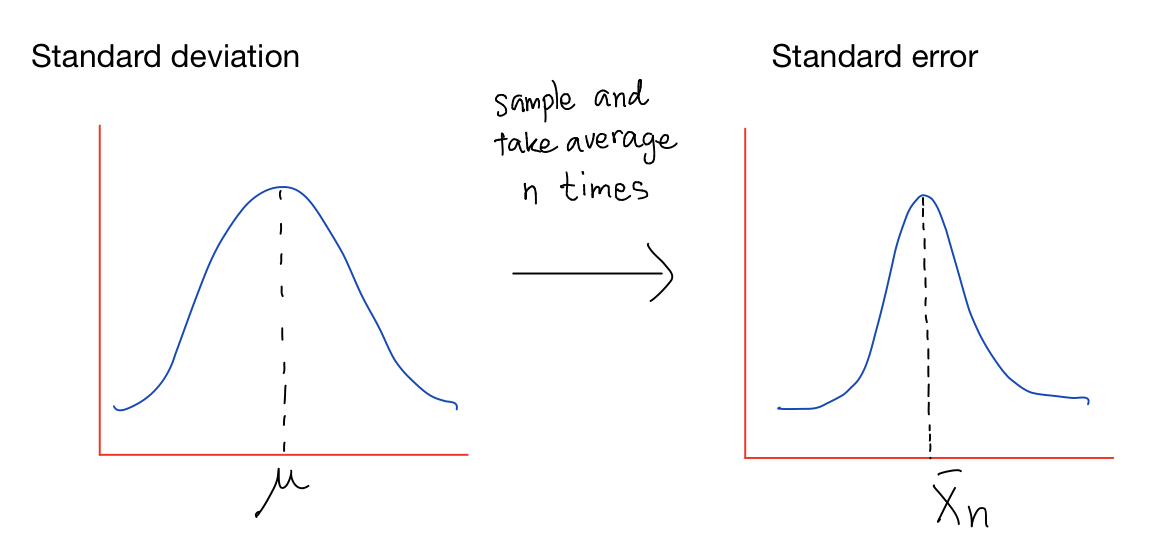
\includegraphics[width=0.8\textwidth]{figures/sd_se.jpg}
    \caption{Comparison between standard deviation and standard error}
    \label{fig:example_figure}
  \end{center}
\end{figure}

Standard deviation is variation in the population which always remains the same, while standard error can be reduced by sampling more samples.

\section{Regression}

A simple definition of regression is to predict some outcomes from some inputs/ features/ predictors.

\begin{align*}
&{\big\{y_i \big\}}_{i=1}^N \text{or} 
 \begin{bmatrix} 
    y_{1} \\
    \vdots \\
    y_{N} 
\end{bmatrix}  \text{are N observations of outcomes (usually scalar values) } \\
&{\big\{X_i \big\}}_{i=1}^N  \text{or} 
\begin{bmatrix} 
    X_{11} & \dots & X_{1K} \\
    \vdots \\
    X_{N1} &        & X_{NK} 
    \end{bmatrix} \text{are N observations of inputs of K dimensions (vector input) }
\end{align*}
\noindent
Regression can be simply put as $\hat{y}_i = f(x_i)$, an output of our predictors is equal to our function of inputs.\\
\underline{Goal}: We want some functions whose output matches the data well. To quantifying 'well', we introduce
\begin{align*}
\mathcal{L}_{i}[f] = (y_i - \hat{y}_i)^2
\end{align*}
called loss function of single data point which is calculated using squared error of actual and predicted outcomes.\\
For the whole data set, we have that
\begin{align*}
\mathcal{L}[f] = \frac{1}{n}\sum_{i=1}^{N}(y_i - \hat{y}_i)^2
\end{align*}
Our goal is to find the function that minimize the loss.
\begin{align*}
f^{*} = \operatorname*{argmin}_f \mathcal{L}[f]
\end{align*}
\noindent
\underline{Motivation}: Imagine data is generated by
\begin{align*}
y_i = f(x_i) + \mathcal{E}_i
\end{align*}
where $\mathcal{E}_i $  is noise/error.\\
\\
\underline{Assumption}: 
\begin{align*}
\mathcal{E}_i \sim \mathcal{N}(0, \sigma^2)
\end{align*}
\noindent
The likelihood of seeing the observed data can be calculated by
\begin{align*}
p(\mathcal{E}_i | f) &= p(y_i - f(x_i) | f)\\
&= \frac{1}{\sqrt{2\pi\sigma^2}}e^{-\frac{1}{2\sigma^2}(y_i - f(x_i))^2} \\
p(\mathcal{D}|f) &=  \prod_{i=1}^{N}p(\mathcal{E}_i | f)\\
&= (\frac{1}{\sqrt{2\pi\sigma^2}})^N \prod_{i=1}^{N}e^{-\frac{1}{2\sigma^2}(y_i - f(x_i))^2} 
\end{align*}
Under what function f is the probability of the observed data maxizimized?
\begin{align*}
f^{*} = \operatorname*{argmax}_f p(\mathcal{D}|f) 
\end{align*}
$p(\mathcal{D}|f)$ is the likelihood, hence $f^{*}$ is called Maximum Likelihood Solution.\\

However, dealing with the product term is unpleasant, but thanks the monotonic characteristic of logarithmic function, maximizing $p(\mathcal{D}|f)$ is equivalent to maximizing $log\; p(\mathcal{D}|f)$
\begin{align*}
log\; p(\mathcal{D}|f) &= \underbrace{-\frac{N}{2} log\; 2\pi\sigma^2}_\text{ const. w.r.t. $f$} - \frac{1}{2\sigma^2}\sum_{i=1}^N(y_i - f(x_i))^2\\
\operatorname*{argmax}_f p(\mathcal{D}|f)  &= \operatorname*{argmax}_f log\; p(\mathcal{D}|f)\\
&= \operatorname*{argmax}_f - \sum_{i=1}^N(y_i - f(x_i))^2 \text{ (removed terms which are constant w.r.t. $f$)}\\
&= \operatorname*{argmin}_f \sum_{i=1}^N(y_i - f(x_i))^2
\end{align*}
Hence, we can achieve the Maximum Likelihood Solution by solving Least Squared Error.\\
\\
How do we search over $f$?\\
We can attempt by making another assumption that f is a linear function.
\begin{align*}
\hat{y}_i = f(x_i;w) = w\cdot x =wx_{i1} + ... + wx_{iK} 
\end{align*}
or as a vectorized notation
\begin{align*}
\boldsymbol{\hat{y}} = \boldsymbol{Xw}
\end{align*}
We want to find $w$ that minimize the squared error.
\begin{align*}
w^{*} &= \operatorname*{argmin}_w \underbrace{\sum_{i=1}^N(y_i - w\cdot x_i)^2}_\mathcal{L}\\
0 = \frac{\partial \mathcal{L}}{\partial w} &= \sum_{i=1}^N 2(y_i - wx_i)(-x_i)\\
&= \sum_{i=1}^N (y_i - wx_i)(x_i)\\
&= \boldsymbol{X^{T}(y-Xw)}\\
\boldsymbol{X^{T}y} &= \boldsymbol{X^{T}Xw}\\
\boldsymbol{w^{*}} &=  \boldsymbol{(X^{T}X)^{-1}X^{T}y}
\end{align*}
It appears that we can solve for $w$ analytically in a closed form solution. However the complexity of inverting a KxK matrix is $O(K^3)$ and use  $O(K^2)$ space making the method not feasible for high dimensional data. Moreover, it is also possible that $\boldsymbol{X^{T}X}$ is not invertible. Therefore, we need to an iterative algorithm to solve for $w$.\\
\\
\underline{Gradient Descent}: Guess and update
\begin{align*}
\text{We update } \;\boldsymbol{w} &\leftarrow \boldsymbol{w} - \eta \frac{\partial \mathcal{L}}{\partial w}\\
&= \boldsymbol{w} + 2\eta \boldsymbol{X^{T}(y-Xw)}
\end{align*}
This method takes $O(KN)$ time per iteration and $O(KN)$ space.\\
\\
\underline{Stochastic Gradient Descent}: Update using $w$ using smaller batch size (or 1 data point)

For stochastic gradient descent, we sample datat to compute gradient. Here is an example of using one data point at a time.
\begin{align*}
\boldsymbol{w} &\leftarrow \boldsymbol{w} - \eta (y_i - \boldsymbol{wx_i}) \boldsymbol{x_i}
\end{align*}
This method only requires $O(mK)$ per iteration where m is the batch size. However, it is more sensitive to the step size, $\eta$.




